\documentclass[conference]{IEEEtran}
\IEEEoverridecommandlockouts
% The preceding line is only needed to identify funding in the first footnote. If that is unneeded, please comment it out.
\usepackage{cite}
\usepackage{amsmath,amssymb,amsfonts}
\usepackage{algorithmic}
\usepackage{graphicx}
\usepackage{textcomp}
\usepackage{xcolor}
\usepackage{array}
\usepackage{xurl}
\usepackage{subfigure}
\usepackage{listings}
\usepackage{multicol}
\usepackage{multirow}
\usepackage{subfig}
\usepackage[utf8]{inputenc}

\makeatletter
\newcommand{\linebreakand}{%
  \end{@IEEEauthorhalign}
  \hfill\mbox{}\par
  \mbox{}\hfill\begin{@IEEEauthorhalign}
}
\makeatother

% Define margins
\def\BibTeX{{\rm B\kern-.05em{\sc i\kern-.025em b}\kern-.08em
    T\kern-.1667em\lower.7ex\hbox{E}\kern-.125emX}}
    
\definecolor{codegreen}{rgb}{0,0.6,0}
\definecolor{codegray}{rgb}{0.5,0.5,0.5}
\definecolor{codepurple}{rgb}{0.58,0,0.82}
\definecolor{backcolour}{rgb}{0.95,0.95,0.95}


% Code coloring
\lstdefinelanguage{custom}[]{PHP}
{
morekeywords={public, class, extends, private, function},
}

\lstdefinestyle{php}{
    morekeywords={function}
    backgroundcolor=\color{backcolour},
    commentstyle=\color{codegray},
    keywordstyle=\color{codepurple},
    numberstyle=\tiny\color{magenta},
    stringstyle=\color{codegreen},
    basicstyle=\ttfamily\footnotesize,
    breakatwhitespace=false,         
    breaklines=true,
    captionpos=b,  
    keepspaces=true,
    numbers=left,
    numbersep=5pt,
    showspaces=false,
    showstringspaces=false,
    showtabs=false,                
    tabsize=2
}
\lstset{style=php}

% Define macros
\newcommand{\authorBlock}[6]
{
\IEEEauthorblockN{#1}
\IEEEauthorblockA{
#2 \\
College of Engineering \\
\it{Department of #3}\\
#4, #5 \\
#6}
}

% Document
\begin{document}


\title{BookMark - Bright Bookshelf}

\author{
\authorBlock{Mathilde Lærke Hansen}{9077620215}{Information Systems}{Copenhagen}{Denmark}{malaha@ruc.dk}
\and
\authorBlock{Sarah Schlegel}{9091820217}{Computer Science}{Paris}{France}{sschlegel@protonmail.ch}
\and
\authorBlock{Anais Zhang}{9088520214}{Computer Science}{Paris}{France}{anais.zhang12@gmail.com}
  \linebreakand 
\authorBlock{Young Ha Hwang}{2017029261}{Information Systems}{Seoul}{South Korea}{dudgk970@gmail.com} 
\and
\authorBlock{Laura Vikke Mårtensson}{9077020219}{Computer Science}{Copenhagen}{Denmark}{lauramaartensson@gmail.com}
}




\maketitle

\begin{abstract}
Nowadays, modern people (employees, students, etc.) lack time for reading books. Although they have the motivation to read, when people are investing time in various activities such as studying, working, or exercising, the time for reading has low priority amongst the 24 hours of a day. For example, even if you want to read a book, the hardships of choosing and purchasing a book yourself is an obstacle to start reading. \\
To meet the aspiration of overcoming these obstacles, we created the application BookMark. BookMark is meant to help the customers manage their bookshelf, either physical or digital, and arrange more time in their daily life to read. BookMark provides a system of reminders to keep track of the books the user is currently reading, and makes the bookshelf management easier by using simple image recognition to search for a book by its cover, barcode, or ISBN number. It automatically sorts the content and providing different pairing options between physical copies, ebooks or audiobooks. By automatizing the usually difficult part of book management, BookMark wishes to let the reader make more space in his or her day to actually read.
\end{abstract}

\subsection*{Role Assignments}
\begin{center}
\begin{tabular}{ | m{1.2cm} | m{1.5cm}| m{4.2cm} | } 
 \hline
 Roles & Names & Task description etc. \\ 
 \hline
 User / Customer  & Young Ha Hwang & Ordinary people fitting in to modern society are main users of the application. We assume that they are willing to read, but that reading priorities are set low due to other activities. To check the sustainability of the application, first, a simple survey was conducted to determine users' time management for reading, if they are currently reading a book and how reading is prioritised in their everyday life. \\ 
 \hline
\end{tabular}
\end{center}

\begin{center}
\begin{tabular}{ | m{1.8cm} | m{1.5cm}| m{4.2cm} | } 

 \hline
 Project manager & Sarah Schlegel & The project manager is in charge of planning, assigning the tasks and is generally in charge of ensuring that the project is moving forward. She will make sure that the team meets the different goals at the right time. She has the responsibility to inform the development manager of any changes regarding the project requirements. \\
  \hline
  Development manager &  Mathilde Lærke Hansen & The development manager confirms the final functions of the software with considerations of the user as the main consumer of the application. The development manager mediates and updates the software developers. If the software does not live up to the users needs and expectations, the development manager will gather more information about the customers and then advise the software developers how to fulfill the needs of the user.\\
  \hline
 Software developer & Anais Zhang \&  Laura Vikke Mårtensson & The software developers reflect on which software system that would fit the best for the application. They analyze, categorize and examine the software and make decisions of which development tools that can be used to implement the applications. They collaborate with the development manager \\ 
 \hline
\end{tabular}
\end{center}



\section{Introduction}

\subsection*{Motivation}
The idea for the BookMark project derives from an observation that many people today don't have the time nor the motivation to read new books as they navigate their fast paced and overstimulated everyday life. Our goal is to provide, with this combination of a bright bookshelf and mobile BookMark application, a simpler way to manage the books people are reading, whether it's by easily swapping from a physical book to an audio book, by reminding the user to read at certain times or by recommending them new books based on their current preferences. \\ \\


This application focuses on making reading more efficient for people and helping them sort and keep track of their books on a physical bookshelf. Today, there is no time in the schedule of most people to read books that are not academic or work related. Also, people who actually manage to find the time to read usually keep a physical bookshelf. They could keep a list of audiobooks and ebooks on their devices, and have their bookshelf right in their pockets, or keep both physical and mobile. For peoples who have a lot on their plates, sometimes they might forget their physical copy at home, or maybe want to do a task while listening to their book. Maybe it would help them to have the ebook and the physical copy, and they'd like to switch from one to the other easily without struggling to remember the correct page between the different versions.\\
BookMark is meant to help with these issues mentioned above. If the users can keep track of their reading, and get reminders of their current position in a book, they can be more eager to pick up their book again. BookMark will help the user put the book back to the correct place in a physical bookshelf and not organize a personalized sorting system. When they're done reading and have to get going, they just have to note their current position in the book in the app, whether it's the chapter or the page they left it, and they won't lose track of their progress in the book. \\ \\

Furthermore, if they have already purchased the physical copy, they can simply scan the barcode, the ISBN number, or even just the cover, and the app will give the user alternative options like if the book is available as an audiobook or an ebook, so that they can read or listen as they prefer. The app will also propose time slots to read when a person has a break in their calendar and propose new books they may like to read next, so that they don’t have to search for books that they might like. The application will get to know the user, and therefore know their likes and dislikes. If they purchase an ebook or an audiobook copy, they can directly start listening to the audiobook or reading the e-book on their phone. This application is available through a simple sign up phase and afterwards the subscriber has their own personal login. A chat feature will also be available as a help to the user if needed. The ambition of BookMark is to assist people with their busy schedule and provide space to read more books at their desired pace.

\subsection*{Problem Statement (client's needs)}
Through a questionnaire, we found out, as suspected, that students feel that they do not have the time to read books in their everyday life. We asked different people questions about their normal life. The biggest feedback from an age group was people between 15-26 (94\%). We asked what they need more of in their life, and the number one answer was: time. Other top answers were money and love.\\
The reasons for reading amongst the questioned people were to learn, for entertainment, or for relaxation. To the question: “What would make you read more books?” The answer “more time” was the most frequent one, but here are some other answers worth mentioning: “more awareness of the books out there (too many to know them all)”, “if finding interesting books didn’t require so much research”, “Easier way to get physical books” or “A better variety of English ones in store”.\\
The tested people usually either read 30 minutes before bed, in the summer vacation (when there is no school or work) or during commute on their phones or with a physical book. Some of them have experience with using audiobooks, but most of them don't. The ones that do listen to audiobooks, do it so that they can do other things at the same time.\\
The survey is only a sample test and we acknowledge that this questionnaire is only a snapshot of reality. We only use the stats as an inspiration for our different features in our application.


\subsection*{Research on any related software}
There are quite a few concepts already on the market, or in progress of development, that resemble online bookshelves or ways to track your reading progress. These range from large physical bookshelves aimed at libraries as the targeted consumer, down to mobile applications which help you to keep track of the books that you are reading or want to read.
\begin{itemize}
	\item RFID smart bookshelf
	\item Smart AI Modular Bookshelf
	\item Goodreads
	\item BookBrowse
	\item StoryGraph
\end{itemize}


\subsection{RFID smart bookshelves} 
This company produces large smart bookshelves that are designed to be used in a library and make work for the employees easier. The bookshelves communicate with a central file management system and works by scanning books in real-time through an antenna array. The system has useful functions such as; easy navigation to books when looked up in the system, generating reports when books are placed on the wrong shelf by a reader or an employee and detecting missing books. These bookshelves and their associated functions are very useful and mostly designed for the needs of huge libraries and professionals who are handling a lot of books. In contrast, our project focuses more on the needs of the private consumer, and is designed to help the individual reader with managing their private book collection.\cite{RFID} \\

\subsection{Smart AI Modular Bookshelf} 
This is a concept developed as a way to help the private book owner to better manage their books. It is a physical smart bookshelf connected to an application, which is then used to manage the book collection. The bookshelf uses image recognition technology to keep track of the books location, and embedded lightbulbs in the bookshelf will light up when searching for a specific book. The application offers functions such as reading project management and book reviews. This product is, at this point in time, only a concept and not an actual product on the market. Our project expands on the idea with additional functionalities and features.\cite{Smartbookshelf}\\

\subsection{Goodreads} 
Goodreads is a website and an application, which is meant to keep track of the books that you’re reading, have read and want to read. The main functionalities of Goodreads are meant to help the user to choose a book to read, with features such as book reviews, personalized book recommendations and insight into what your friends and the rest of the Goodreads community is reading. \cite{Goodreads}\\

\subsection{BookBrowse} 
BookBrowse is a book recommendation website who offers excerpts of books to skim just as you would when you browse for books in a library. You can also find Independent and in-depth book reviews, as well as personalized book recommendation and a bookclub subscription. \cite{Bookbrowse}\\

\subsection{StoryGraph} 
This application offers you personalised book recommendations, as well as tools to keep track of your reading progress and statistics. If you have a Goodreads account, you can import your data into the application. \cite{Storygraph} \\

\section{Requirement Analysis}

\subsection{Log-in}
When the user download the app, the main page shows two inputs for the email and password to sign in, if user already has an account. If they don't have an account, they can create one with the \textit{Sign Up} button below the login form on the main page, which will redirect them to the sign up page. Finally, a smaller link can lead them to the account recovery page in case they forgot their password.\\
For the login process, the software looks into the database to find the matching combination of username and password or email and password for a user. After logging in, the user is redirected to his main page, \textit{My BookMark}.\\

\subsection{Sign up}
Membership requires basic information such as a unique username, a valid email, a password, and an optional phone number for password recovery. The password has to be at least 8 characters long, with one uppercase, one lowercase, one number and one symbol.\\
The app also requires the user to agree with the terms and conditions, and optionally to subscribe to the newsletter. The terms and conditions are displayed in a scrollable pop-up that allows the users to read them without losing the data they've already input in the form.\\
The sign up process then creates a 8-digit token and sends it to the user in a confirmation email, in clear and in a hyperlink. The hyperlink leads to a confirmation page that will display the success of the confirmation.\\
Once the email has been verified, the user can log into the app. For the first connection, the user must choose at least 3 genres of books he or she likes to set as reading preferences for the recommendation algorithm.\\


\subsection{My BookMark}
The home page of the app functions as a 'hub' from where you can access all the different features of the application. The bottom menu is composed of five buttons, each represented as a symbol:
\begin{itemize}
	\item Home: brings the user back to the home page
	\item Library: takes the user to the list of books (\textit{My Bookshelf} page)
	\item Add: goes to \textit{Add a book} page
	\item Statistics: brings the user to his \textit{Statistics} page
	\item Account: goes to the \textit{User account} management and settings page
\end{itemize}

The home page in itself consists of a preview of the user's shelves and categories. By clicking on each element, the user opens a more detailed page of the shelf or category, listing all the books that it's referencing and his current progress in those books. When he clicks on one of them, he triggers the \textit{Book view}.\\

\subsubsection{Add a book}\hfill\\

The user clicks the central + button in the bottom menu to add a new book. This action displays a pop-up to ask him if he wants to enter the book manually or use the camera to scan the book's cover, the ISBN number or the barcode.\\
If he selects the scan option, the app opens the camera and the user scans the book. If it's the cover, the image is decomposed using an image recognition library to figure out the book title and pair it with a book in the user's collection or a book in the internet databases. If it's a barcode or an ISBN number, the app searches in external APIs to find the book reference through the given number. Once the app has found a matching book by image recognition or by an external request, it asks the user to confirm that it's the correct book and if he wants to add this book to his library. If yes, the book is added to the library and assigned to a shelf on the bookshelf. The shelf lights up to show the placing of the book.\\
If the user has selected the manual entry of the book, he is prompted to enter the book title and author. The book is then searched on the Internet and the ISBN and book title are displayed to the user to ask him if it's the correct book and if he wants to add it. Then we repeat the same process as for the scan option to assign the book to a shelf.\\

\subsubsection{My Bookshelf}\hfill\\

This page displays a list of the books and ebooks owned by the user sorted depending, listing them in different categories:
\begin{itemize}
	\item New Arrivals: shows the two most recently added books.
	\item Currently reading…: shows the books the user is currently reading, sorted by latest reading update.
	\item Wishlist: shows the books the user has added to his wishlist from the recommendations.
	\item Recommended: recommended books depending on what the user has already read. Clicking on this list redirects to the \textit{Suggested books} page.
	\item All books: displays a list of all the books depending on the user's sorting parameters (author, title, genre). The sorting type can be selected in the \textit{User account} settings.
\end{itemize}
Each category at first only displays 4 books, but it can be expanded to display the complete list.\\
The page also has a search bar to find a book easily. When the user starts inputing text in the search bar, the app searches for the book depending on the title or author's name in the user's bookshelf, hiding the rest of the categories. If the book isn't in the user's bookshelf, the search shows 'No results' and proposes to search for the book on the Internet and in the book database.\\
By clicking on a book, the user toggles the \textit{Book view} for this specific book.\\


\subsubsection{Book view}\hfill\\

The book view displays the book data: title, author, eventual number of pages, shelf position, current labels, reading status and notes. If he clicks on a little bookshelf icon atop of the page of a book of which he owns a physical copy, the physical bookshelf will light up the shelf on which the book should be stored, depending on the current sorting parameters.\\
The user can update the following things on the book:\\
\begin{itemize}
	\item The label assigned to the book (read, not read, currently reading);
	\item His reading status (current page or chapter number);
	\item His personal annotations, whether they're global or whether they are related to a specific page or chapter;
	\item His personal rating, with zero to five stars;
	\item Specific reminders to read this book if he's currently reading it.
\end{itemize}

If the user wants to remove the book from his app library and from his bookshelf, he can click on a button at the bottom of the Book view. A popup window will appear to ask him if he's certain to want to remove this book from the bookshelf and from the library. The book will then be removed from the user's collection and from the positioning in the physical bookshelf.\\

\subsubsection{Suggested books}\hfill\\

A separate page displays the recommended books for the user depending on the books he already owns. For this, we will design a personal machine learning algorithm inspired by popular suggestion algorithms like Netflix's, YouTube's, Instagram's or Amazon's.\\
The page consists of a list of books and covers. If the user clicks on a book, it will toggle a simplified book view with the title, author, number of pages, and a + button to add the book to his bookshelf.\\

\subsubsection{Statistics}\hfill\\

The statistics page displays information about the user's reading history and bookshelf data in the form of graphs and numbers. The statistics displayed are the following:
\begin{itemize}
    \item Last books read: The names and links to the 3 books that were updated the most recently, whetter read or currently reading.
    \item Graph of books read: A bar chart displaying the number of books read in the last 3 months.
    \item Bookshelf completion: The number of books read over the total number of books in the bookshelf.
\end{itemize}
That way, the user can keep track of his current progress.

\subsection{Physical Bookshelf}

The physical bookshelf comes in various sizes and colors, but in a common simple design that appeals to many different types of people. The bookshelf will need to be plugged into a power source in order to function and be able to connect with the associated app. On each shelf there is a LED band that can light up when triggered by the app.\\

\subsubsection{Connect to bookshelf}\hfill\\
In the user settings, there's an option titled 'Bookshelf' to configure the user's physical bookshelf.\\
If the user is not yet connected to the bookshelf, when he selects this option, a large pop-up appears. If the Bluetooth is off, it asks the user to turn off the Bluetooth. When the Bluetooth is on, it starts searching for devices ready for connection, and displays only the nearby BookMark bookshelves. If the user clicks on one of them, it prompts him for a connection confirmation. Multiple users can be connected to the same bookshelf.\\
Once the user's account is bound to the physical bookshelf, when the user clicks on the Bookshelf option in the settings, the page displays the informations of the bookshelf. These include the id number, the dimensions, the number of shelves, the number of books in the bookshelf, the number of audiobooks and ebooks and the sorting and sub-sorting categories.\\
The sorting categories are two dropdowns that allows the user to select between sorting by title, author, genre or none. If the user changes the sorting category, a pop up is displayed to confirm the change and recompute all the sorting in the bookshelves. page will display a graphical preview of the bookshelf and all the books in the right order.\\

\subsubsection{Disconnect from bookshelf}\hfill\\
At the bottom of the bookshelf information page, there's a button to disconnect from the physical bookshelf. If the user clicks it, it prompts him for confirmation in a pop up window. When the user disconnects from the bookshelf, the books on his account are preserved but the shelving and the sorting in the bookshelf are deleted.\\
If the user is the only user connected to the bookshelf, the app asks him if he also wants to delete all the bookshelf recordings. If he does, all the related data to this bookshelf in the database will be dumped.\\

\subsubsection{Book lookup}\hfill\\
When the user scans a book that is already in his collection or selects a book from the list on the app, the bright bookshelf lights up the correct shelf to highlight the correct position of the book depending on sorting. Or, the other way around, the user can select a book in the app and click on a button and it will light up the shelf on which the book should be stored.\\

\subsubsection{Bookshelf sorting}\hfill\\
In the settings, the user can view the current sorting of the shelves in two dropdowns: sorting and sub-sorting. If none is selected, the books are just stored by date added. If a sorting (by genre, author, title, etc.) is selected, then in the All Books category of \textit{MyBookmark}, the book previews will be rearranged depending the sorting category.\\
By clicking on a shelf or in the sorting menu in \textit{MyBookmark}, the user can rearrange the bookshelf sorting manually or select a new sorting category. \\
If he wants an automated sorting, he selects the main sorting category (genre, author, title, etc.) and the app will compute the best rearrangement of the books depending on the books available in physical copies, the main sorting category and eventually another sub-sorting option (sort by author then book title for example).\\
If he wants to sort them manually, he can move the books from shelf to shelf by clicking on a button or drag-and-dropping them from shelf list to shelf list.\\


\subsection{Settings}\hfill

In the settings page, the user can change the language of the app, or change the mode of his screen (dark or light mode) and set all the reading notifications. A switch will be available for the user if he wants to activate or deactivate reading notifications. They are activated by default.\\

\subsubsection{User account}

In the user’s account page, the user can check their personal information like username, phone number or email. They can also change these informations.\\
To change their email, the app requires the user to enter their password. If they changes their email, it will trigger the sending of a confirmation email to the new email; until then, the new email will not be used.\\
For changing their password the users must put their current password and then the new password twice to confirm the newest one. As for the signup, the new password must be at least 8 characters long, with one uppercase, one lowercase, one number and one symbol.\\

\subsubsection{Account delete}\hfill\\
At the bottom of the account page, there's a button for deleting the account. Clicking on that button toggles a confirmation popup to ensure the user really wants to delete their account. Then, the user has to click the link received in a confirmation email to terminate their account. Their preferences, informations and data stored will be deleted from the database and the physical bookshelf will be unbound from the user's account.\\

\subsubsection{Reading frequency}\hfill

The user can change their reading frequency with 2 possibilities: per day or per week.\\
There is a button to let the user choose their frequency of reading.\\
If a user chooses to read every day they must specify the hour that they would like to read.\\
If a user chooses to read every specific day in a week they must choose which days and time they wants to read.\\
According to their choice a pop up will appear to help users to select time or date and time.\\
Default setting for reading time is automatically set every day at 9am.\\

\subsubsection{Log out}\hfill\\
The logout button at the bottom of the user's settings list. To log out user just clicks on the button and a pop up appears to confirm the log out. The user is redirected back to the \textit{Log in} page.\\


\subsection{Audiobook/Ebook binding}
In their personal account, the user can bind their Amazon, Kindle, Audible or other reading accounts to sync their libraries.\\
When their libraries are synced, the user can toggle the opening of another app (Kindle, Audible, etc.) to jump directly to the audiobook or ebook depending on their current position:\\
For an audiobook, it plays the audiobook from the saved timestamp\\
For the ebook, it opens to the correct page in the reading app.\\


\section{Development Environment} 
\subsection{Choice of software development platform}

Our development environment will be mostly UNIX based and Apple oriented since most of us have Apple products such as iPhones or MacBooks. That way, we can use tools that are already provided in the Apple development environment, such as the Xcode IDE. Xcode is created by Apple and therefore optimized to create application for OS devices, with the possibility to run the app on a simulator or on a connected iPhone to see the progress, and it comes with built-in tools for iOS and MacOS development.\\
The code and documentation will be held on a public GitHub repository to grant easy access and have a good overview of the project progress.\\ 

\begin{center}
\begin{tabular}{ | m{1.9cm} | m{5.7cm}| } 

\hline
Tool/language & Reasoning \\
 \hline
 Swift 5.5 &  Swift is a programming language created by Apple inc. in 2014 and is designed to be powerful and intuitive when writing code and applications for Apple OS devices. It has an intuitive syntax, close to C-based languages, and it can be used in combination with Xcode to preview the application interface while it is developed. We will use this language to create the front-end of the application with the default 5.5 version which is included in Xcode.\\
  \hline
 OVH VPS (Apache) &  The server is be a Virtual Private Server hosted on by OVH. It is configured with a Debian 10 OS, and Apache 2 for web hosting, and has basic access as well as a root access for doing all the configuration. The MySQL database is set up directly on the server.\\ 
 \hline
 MySQL & We need a database to manage the data related to books, users and bookshelves. MySQL is an open-source database management system, widely used and popular for handling small and big databases, easily installed on a server and is used in combination with the SQL language in order to manage the data.\\
 \hline
 \end{tabular}
 
 \begin{tabular}{ | m{1.9cm} | m{5.7cm}| } 
 \hline
 PHP/JS & The backend website for management, whether it's users, books or bookshelves, will be in PHP and JS. PHP is the most common scripting language for web development, along with JavaScript, and the combination of both allow for a fast website with asynchronous queries and dynamic updates. We will especially be using PHP as the API language since it is one of the easiest ways to connect to a database and fetch or send data. As PHP can be object-oriented, its inheritance principles will greatly simplify the building of database queries.\\
 \hline
 Python & Python is a high-level general-purpose programming language which supports both object-oriented and functional programming. Many public Python libraries focused on machine learning and AI are available, which is why we chose this language to create the AI part of our project. \\
 \hline
 
\end{tabular}
\end{center}
\hfill

\subsection{Cost Estimation}
\hfill

\begin{center}
\begin{tabular}{ | m{4.6cm} | m{3cm}| } 

\hline
Resource & Price (Won) \\
 \hline
 Web Server  & 23.571 \\
 \hline
 Apple Developer License & 116.676 \\
 \hline
 
\end{tabular}
\end{center}

\hfill
\subsection{Software in use}
\subsubsection{Goodreads}\hfill\\

Goodreads has an application on the market that includes some of the same functionalities as our project, but does not offer the option to connect with a physical bookshelf. Goodreads has a section called 'My Books', as seen in Figure \ref{fig:goodreads} which is designed to keep track of the books in the users collection, and offers the option to use the camera to scan the physical books in your collection. BookMark will offer a similar book management system, but will be synchronized with the users books placement in the physical bookshelf to create an even more powerful organizing tool for the user. \\


\begin{figure}[h]
    \centering
    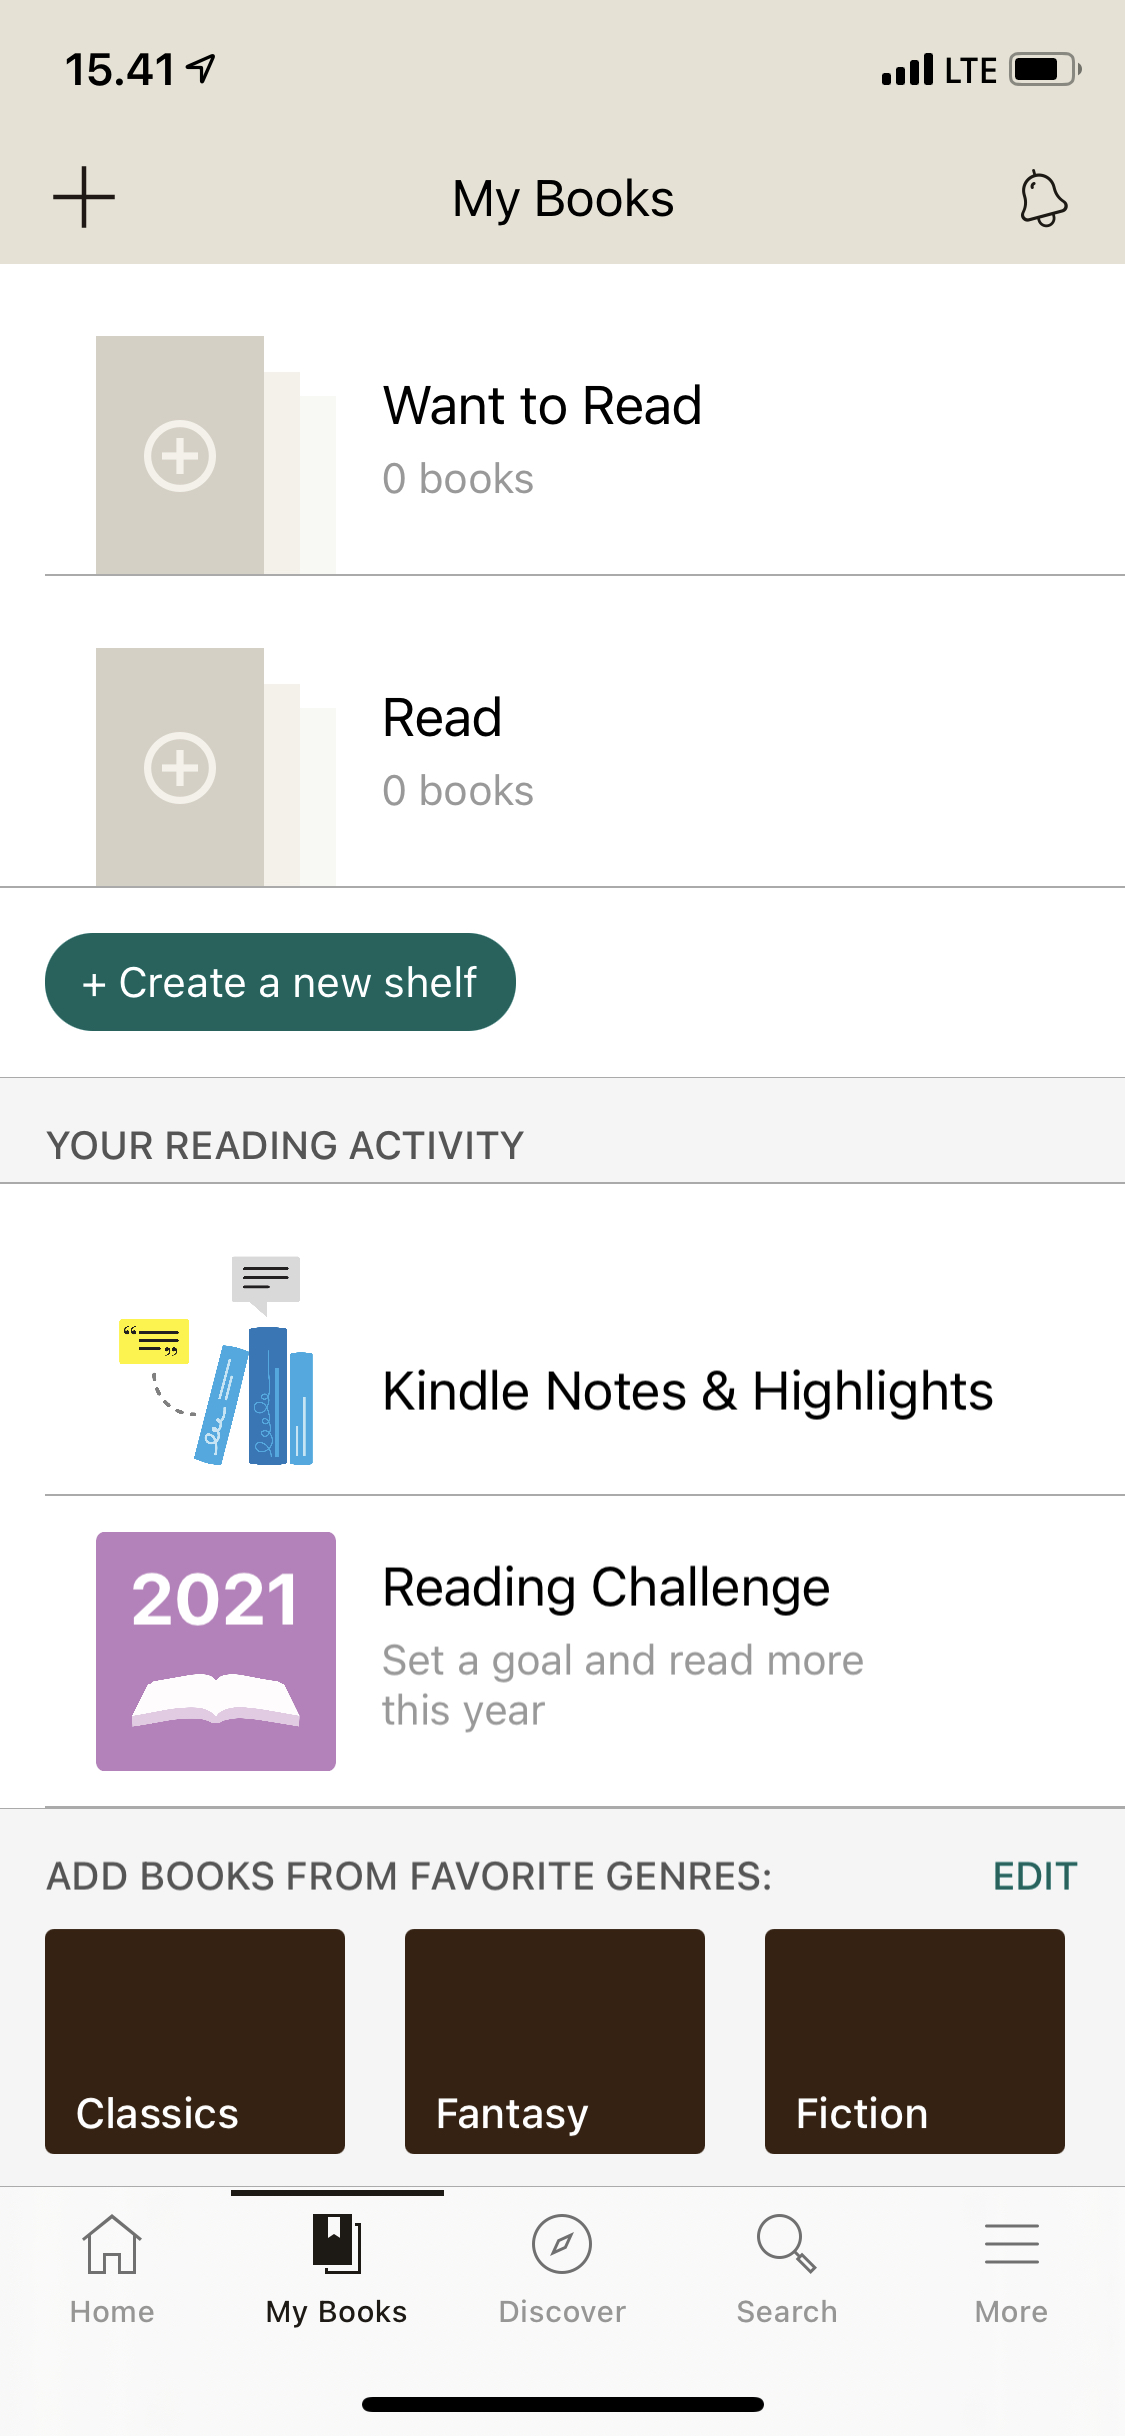
\includegraphics[width=3cm]{Resources/Software/goodreads.jpeg}
    \caption{Goodreads app: My Books}
    \label{fig:goodreads}
\end{figure}

\subsubsection{Amazon API}\hfill\\

The application offers the functionality of 'Add a book' to the user's virtual bookshelf, which requires the app to be able to access some sort of database of books. For this purpose, BookMark will make use of an Amazon Books API for searching and looking up books available in Amazon. For the scope of this project, Amazon currently offers free access to a HTTP or REST API, which can be accessed with the help of a Lambda function for the backend. \\
  

\subsection{Task Distribution}
\hfill

%(If you want, you can provide this later at the nextphase-design)
%       Which member is responsible for what? 

\begin{center}
\begin{tabular}{ | m{3.5cm} | m{4.1cm}| } 

\hline
Name & Responsibilities \\
 \hline
 Sarah Schegel  & ? \\
 \hline
 Mathilde Lærke Hansen & ? \\
 \hline
 Young Ha Hwang & ? \\
 \hline
 Anais Zhang & ? \\
 \hline
 Laura Vikke Mårtensson & ? \\
 \hline
 
\end{tabular}
\end{center}

\section{Specifications}

\subsection{Database}

\begin{figure}[h]
    \centering
    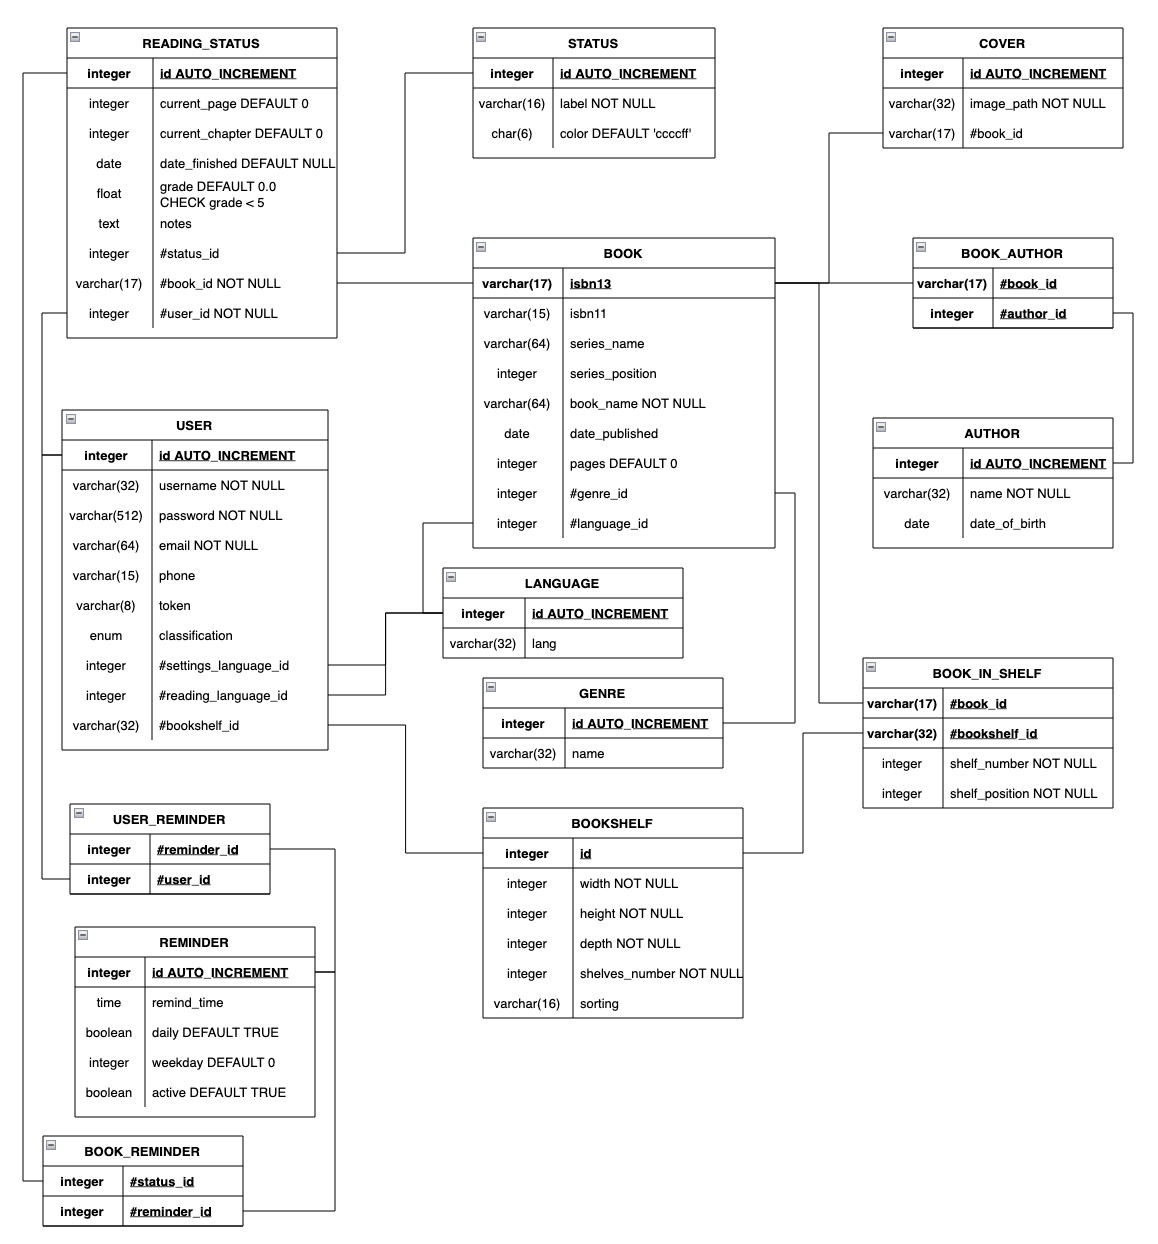
\includegraphics[width=9cm]{Resources/Specifications/LDM.png}
    \caption{Logical Data Model\cite{LDM}}
    \label{fig:ldm}
\end{figure}

Figure \ref{fig:ldm} shows the Logical Data Model of the database. The primary keys of the tables are in bold, the types of the columns are on the left side and the names and constraints (check values and default values) of the columns are on the right side. The foreign keys are identified with a \# and linked to the table they are referencing.
The main tables of our database are the 'user', 'book', 'bookshelf' and 'reading\_status'. Along with the associative tables and the other tables for satellite data, these four tables are the ones that will be used the most for managing our users and our bookshelves.

\subsection{Log-in}

The Log-in page as shown in figure \ref{fig:login} is the first page that the user will be met with when they have downloaded the application and opened it for the first time. The user will have to input username and password using the mobile keyboard, and the application will (use API?) to request the database if such a user exist, when the user presses 'Log-in'. If in existence in the database, the user will be guided to the home page, e.g 'My Bookmark'. If the user does not already have an account, a button called 'create' is displayed in the bottom of the screen, which will guide the user to the sign-up page. Lastly, if the user has forgotten their password, they have the option to request a new password from the log-in page.

\begin{figure}[h]
    \centering
    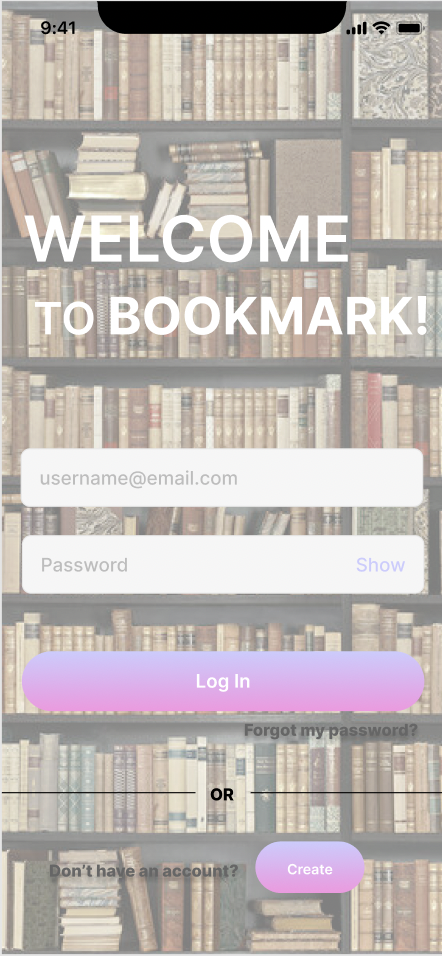
\includegraphics[width=3cm]{Resources/Specifications/Login.png}
    \caption{Log-in page}
    \label{fig:login}
\end{figure}

\subsection{Sign-up}
If the user does not already have an account and have therefore been guided to the sign-up page, as seen in Figure \ref{fig:signup} there are several datapoints that the user will have to input in order to be created in the database. An username, Email, Phone number and sufficiently secure password should be inputted. Moreover, the user has to agree to the terms and conditions of the applications, of which can be accessed and read through a hyperlink. Lastly, the user has the opportunity to sign up for a newsletter, where they will be registered in a mailing list and send regular emails with personalized book recommendations and etc. based on their data. \\
After the user's sign-up details has been approved and created in the database, the user will be guided to a new page, as seen in Figure \ref{fig:categories} where they have the option to choose their favorite genres such that the recommendations and search results in the app will become more relevant to the users personal preferences. 


\begin{figure}[h]
    \centering
    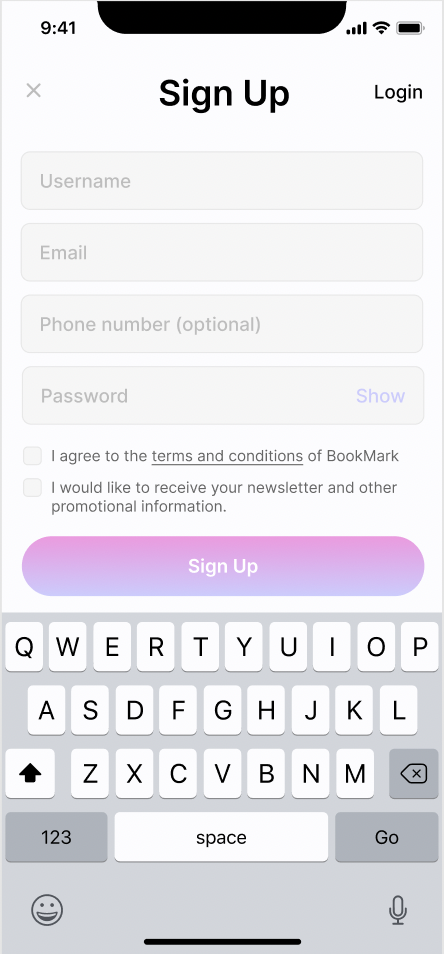
\includegraphics[width=3cm]{Resources/Specifications/signup.png}
    \caption{Sign-up page}
    \label{fig:signup}
\end{figure}

\begin{figure}[h]
    \centering
    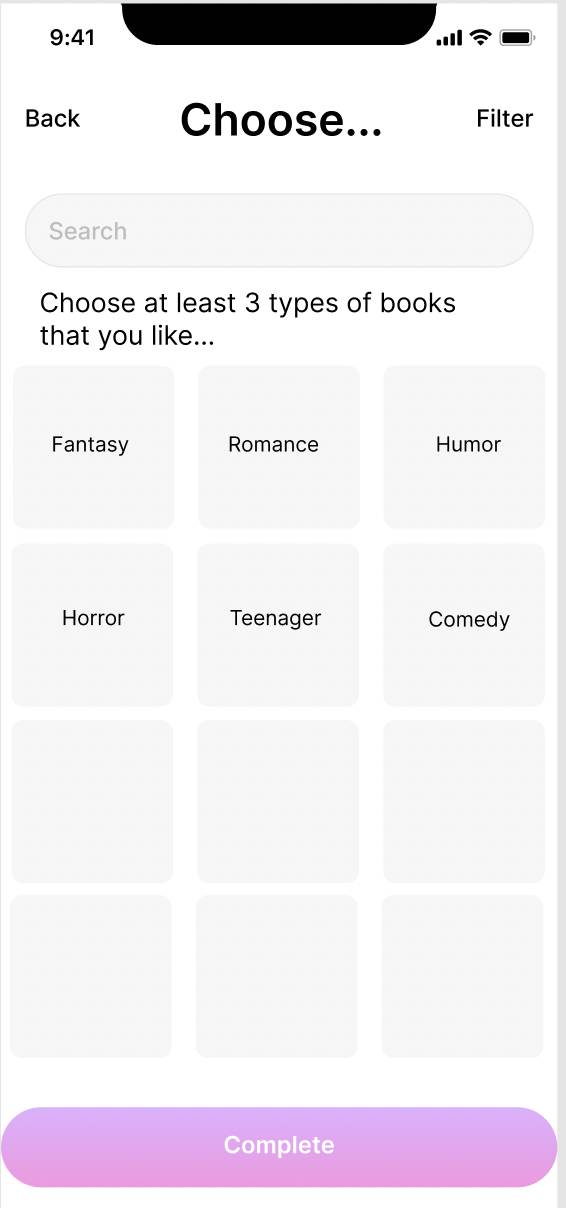
\includegraphics[width=3cm]{Resources/Specifications/categories.png}
    \caption{Preferences page}
    \label{fig:categories}
\end{figure}



\subsection{My BookMark}
The page 'My BookMark', as seen in Figure \ref{fig:mybookmark} is the first page the user will be guided to when they are already logged in and opens the app. It is the user's personal page where they will have the option to upload a photo of themselves in order to personalize their page, and they will be able to access different main functionalities of the app. At the top of the page, the user will have the option to press a 'back' button, which will guide them to xxxx, and a '+' button which will guide the user to the 'Add a book' page. \\

'My Bookmark' will also preview of the user's current bookshelf with images of the bookcovers. They will have the option to view all the books in their collection from the the default 'My books' view, as well as a views called 'Now reading' which will provide different options if clicked on a book, as seen in Figure \ref{fig:book}. The user will be able to see their reading progress, rank the book, delete the book from their collection and keep reading the book. If the user chooses to 'Keep reading' the book will either be opened as an Ebook, or the physical bookshelf will light up where the physical book is stored.  \\

At the bottom of the page, which will be available from most pages within the application, the user has access to the four main sections of the application, as well as a '+' button for quick access to adding a new book to the user's collection. The first button will guide the user to the main page, the next to the 'My Bookmark' page, the third to the reading statistics page, and the last to the 'User Account' page.

\begin{figure}[h]
    \centering
    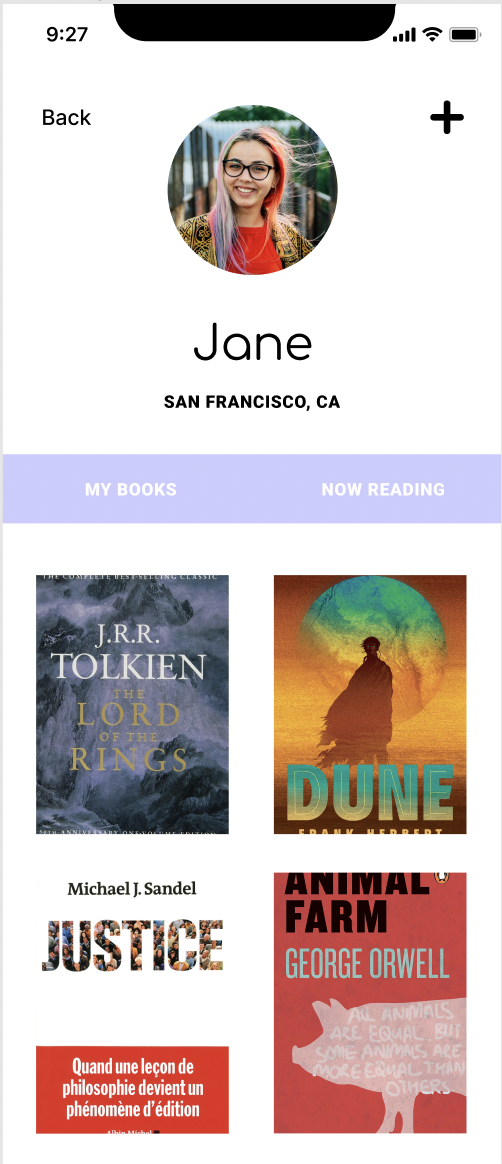
\includegraphics[width=3cm]{Resources/Specifications/mybookmark.png}
    \caption{My Bookmark page}
    \label{fig:mybookmark}
\end{figure}

\begin{figure}[h]
    \centering
    
\includegraphics[width=3cm]{Resources/Specifications/book.png}
    \caption{My Book page}
    \label{fig:book}
\end{figure}

\subsection{Add a book}
When the user press a '+' button anywhere in the app, they will be met with a pop-up asking if they wish to add a physical book or an ebook. If they choose ebook, they will be be shown a 'search' page which will show updated suggestions based on what the user inputs in the search field. When the user has located the book they want to add, they will be guided to the 'Add a book' page, as seen in Figure \ref{fig:addabook}. \\
This page previews information about the book, as well as ratings and reviews from other users of the application. The user will press the button 'Add My List' to add the book to their bookshelf in My Bookmark.\\

If the user chooses to add a physical book, they will be guided to a new page using the camera in order to be able to scan the cover, ISBN or barcode of the book. Then the book is automatically added to the user's bookshelf in My Bookmark, and the physical bookshelf is updated to recognize this book as a part of its collection as well.

\begin{figure}[h]
    \centering
    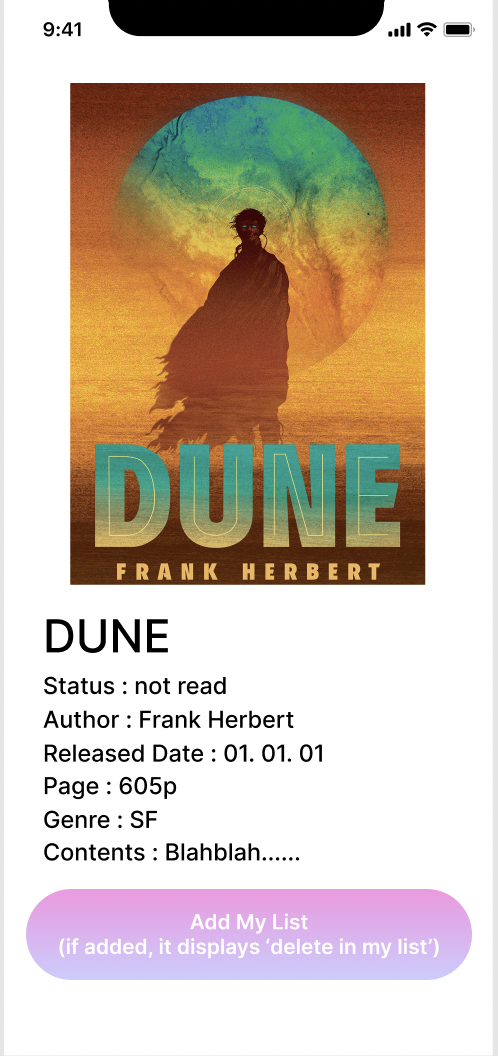
\includegraphics[width=3cm]{Resources/Specifications/addabook.png}
    \caption{Add a book page}
    \label{fig:addabook}
\end{figure}

\subsection{Main page}
The main page, as seen in Figure \ref{fig:mainpage}, functions as a mixture between an overview and a discover page, where the user will be able to view the books they are currently reading as well as discover new books, which the application suggests based on personal preferences. There will be recommended books based on the user's preferred genres, books similar to the one the user has already read and New Arrivals which fits the user's preferences. \\

The user will also have access to a search function they can use based on book names and authors, which will search the database for the requested book or books.\\
At the top left of the page, the user user will have the opportunity to to log-out of the application and at the top right the '+' button us present, guiding the user to the 'Add a book' page.

\begin{figure}[h]
    \centering
    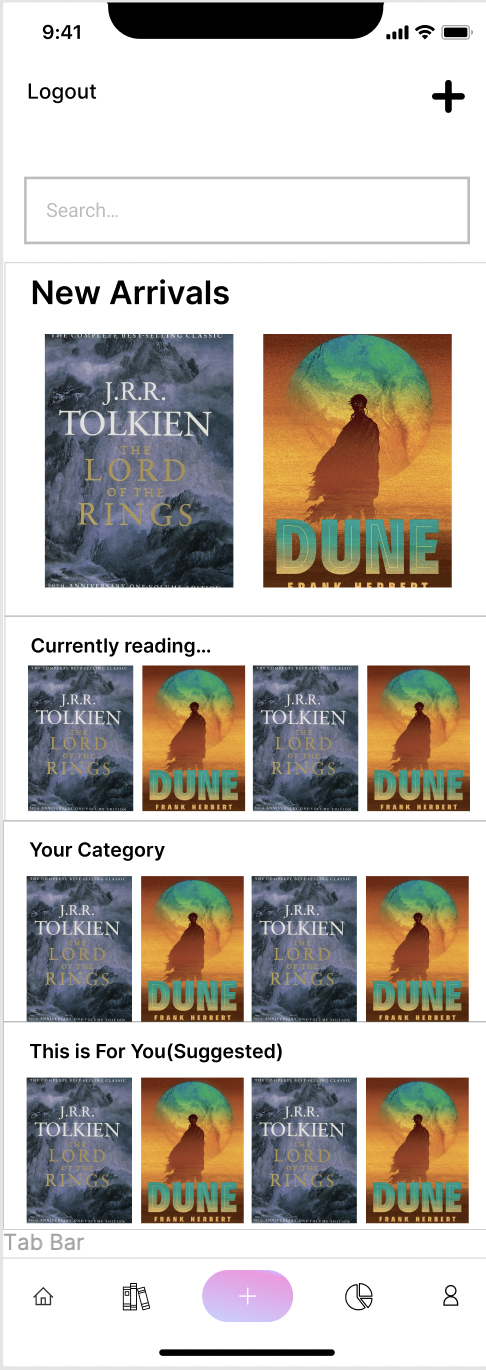
\includegraphics[width=3cm]{Resources/Specifications/mainpage.png}
    \caption{Main page}
    \label{fig:mainpage}
\end{figure}

\subsection{User Account}
The user account page, as seen in Figure \ref{fig:useracc}, previews the user's personal information as well as the option to change any of the information, or delete the account entirely. At the top of the page, the user has the option to log-out of the application or to access the 'Settings' page of the application, as seen in Figure \ref{fig:settings}. \\

The settings page offers the user to customize different aspects of the application, such as a light/dark mode, language options and which notifications the user prefers to receive.


\begin{figure}[h]
    \centering
    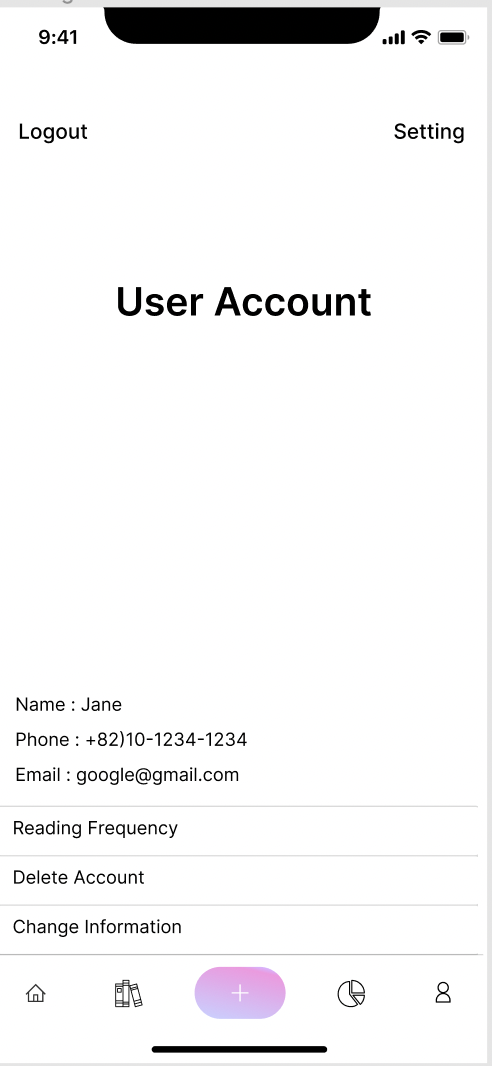
\includegraphics[width=3cm]{Resources/Specifications/useracc.png}
    \caption{User Account page}
    \label{fig:useracc}
\end{figure}

\begin{figure}[h]
    \centering
    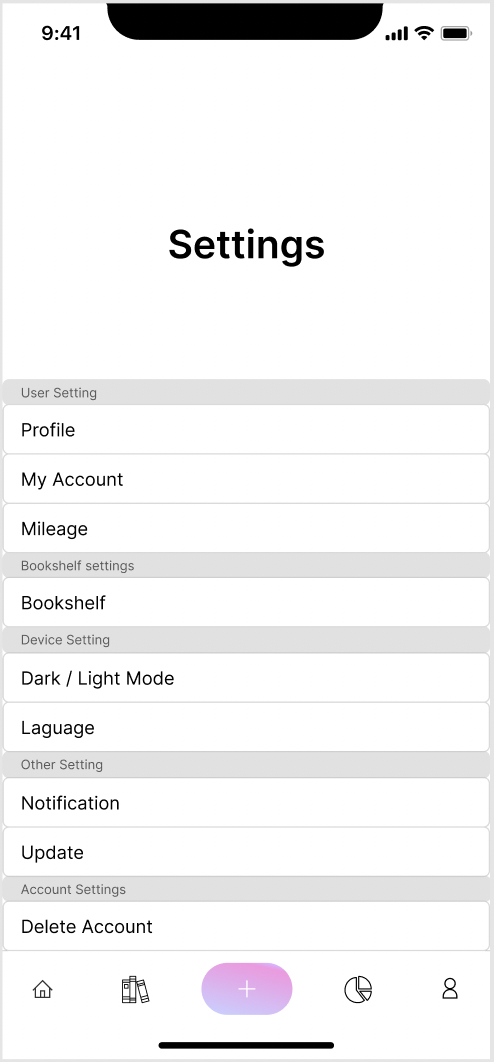
\includegraphics[width=3cm]{Resources/Specifications/settings.png}
    \caption{Settings page}
    \label{fig:settings}
\end{figure}

\subsection{Statistics}


\section{Architecture Design \& Implementation}
\subsection{Overall architecture}

%Provide a figure of overall system architecture (modules or software components, any relationships between)

%Your figure should include the following (recommended, feel free to choose any way that you like):
%    * Box –a module or software component. Each box has a title, description, and its required classes (we will discuss more in class)
%    * Directed edge –relationship between the modules describing which module is used where
%    * Labels –functions or relationship counts on top of each edge (optional)

BookMark is divided into two main modules: the frontend and the backend (see Figure  \ref{fig:architecture}). The frontend is the application in Swift, hosted in its own git repository, and available on iOS devices. This application, when connected to the internet, sends HTTP requests, with a JSON body most of the time, to the server to fetch data.

\begin{figure}[h]
    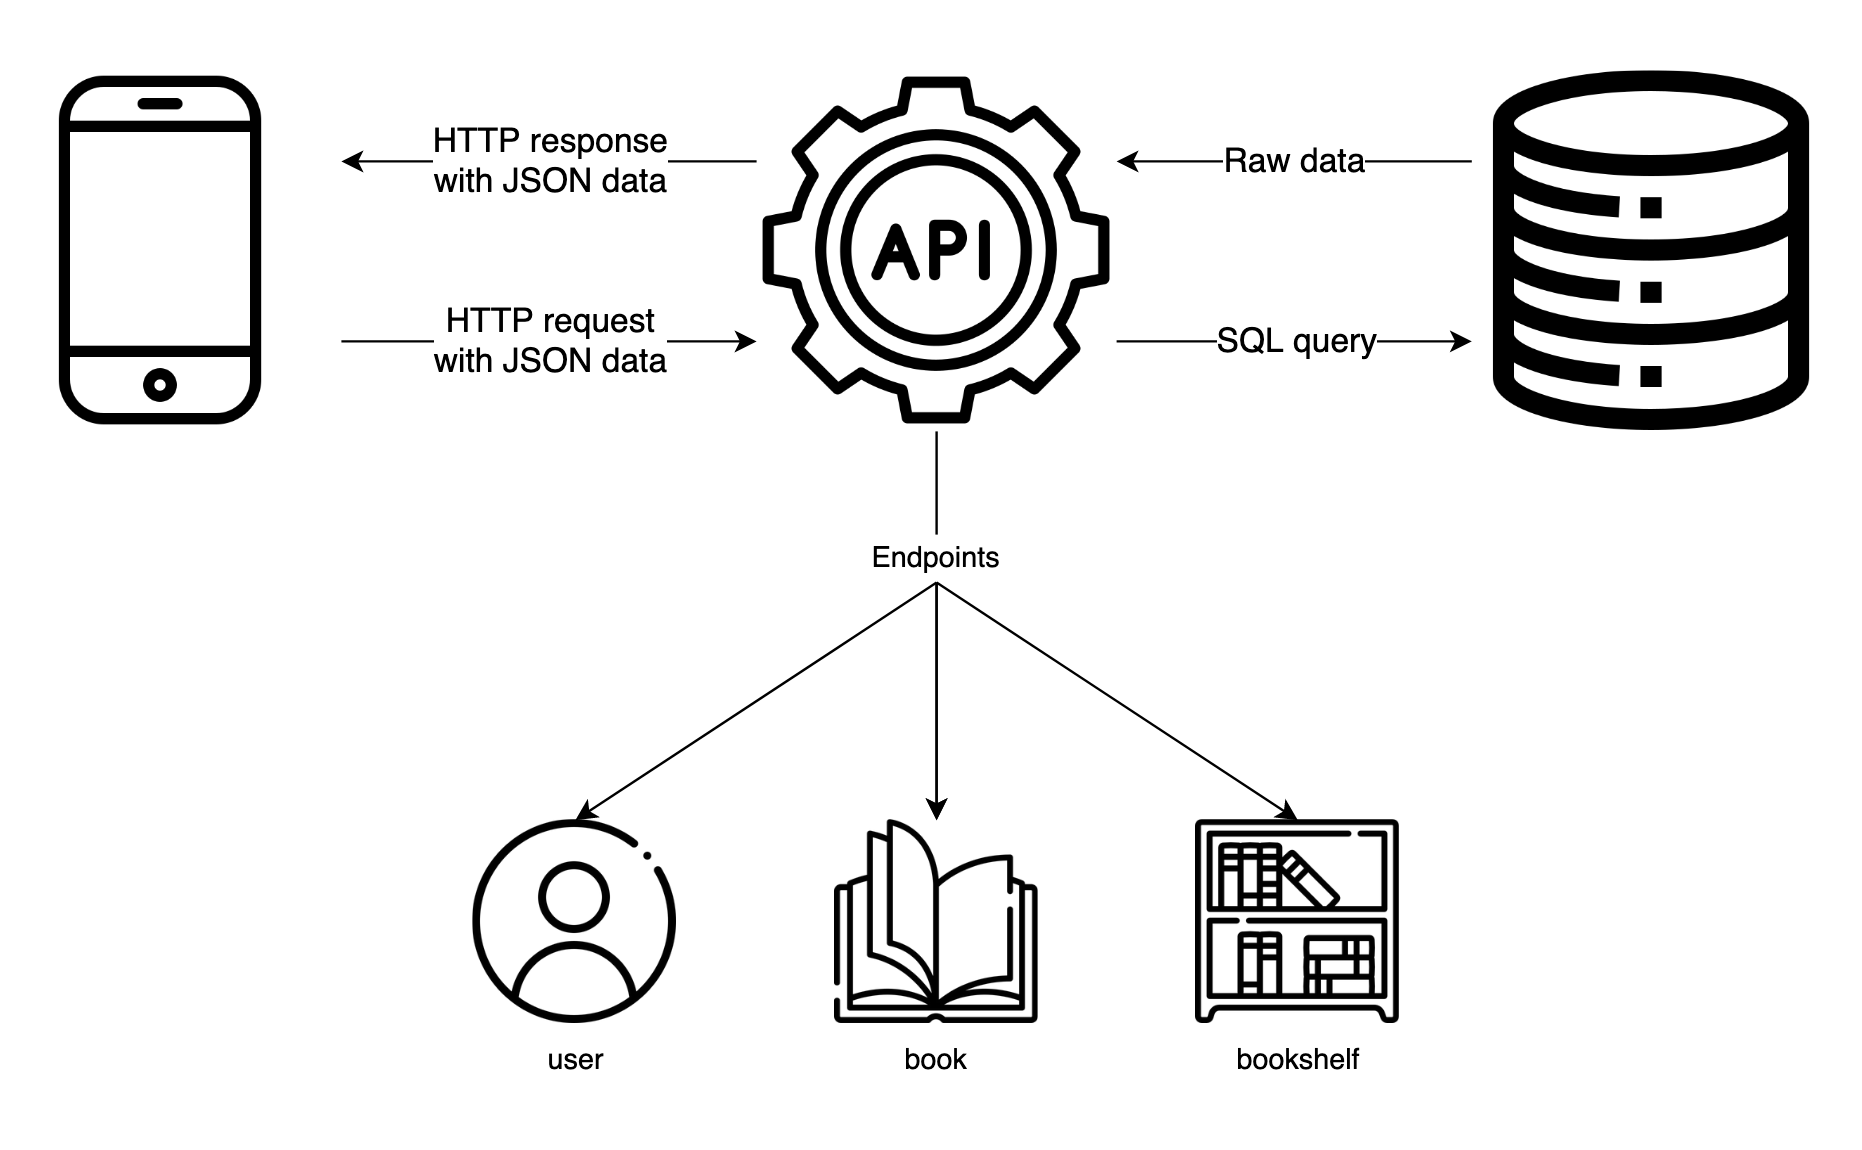
\includegraphics[width=\columnwidth]{Resources/Architecture/Overall.png} 
    \caption{Overall architecture}
    \label{fig:architecture}
\end{figure}

The backend server has three main endpoints for the API : book, user and bookshelf. Those endpoints are respectively available by querying the \textit{/api/book,} \textit{/api/user} and \textit{/api/bookshelf} of the BookMark URL. The rest of the URL parameters are used to specify the actions or the data required for the request. For example, \textit{/api/book/id/0439358078} will get the data of the book that has the ISBN13 "0439358078", whereas \textit{/api/book/search/Harry} will search for all books that have "Harry" in their title or as their author. Most of the time though, the data is sent in JSON in the body for more security.\\
Once the request has gotten to the server, the API on the server processes the data and creates an SQL request to send to the database. Then, it connects to the database, which is hosted locally, and fetches the raw data. This data is then processed again to be output in a JSON format readable for the Swift app.



\subsection{Directory organization}

\begin{center}
\begin{tabular}{| m{3cm} | p{4.6cm}|} 

\hline
\textbf{Directory} & \textbf{Contents} \\
 \hline
 /BookMark  & Root directory, contains the .git* files and all subsequent folders.\\
 \hline
 /BookMark /Documentation & Documentation folder containing the LaTeX file and the PDF, as well as a subfolder \textit{/Resources} for the images used in the documentation. \\
 \hline
 /BookMark /Resources & Folder containing all exterior data such as the LMD, the database scripts. \\
 \hline
 /BookMark/Sources /AI & Code directory, contains the Jupyter notebook for the AI recommendation algorithm. \\
 \hline
 /BookMark/Sources /BookMarkAPI & Code directory, contains the backend code for the server. This directory is a git submodule, so it is managed and versioned independently of the global /BookMark directory. This is also the root directory for the website. It is built on an MVC pattern, and so divided into three main folders: \textit{controllers}, \textit{views} and \textit{api}. The controller files do the redirection and the URL parsing, while the views display the output, and the api files act as "models" and query the database. \\
 \hline
 /BookMark/Sources /BookMarkSwiftApp & Code directory, contains the code for the Swift application. This directory is an Xcode project as well as a git submodule, and just like the BookMarkAPI, is versioned independently of the rest of the git directory.\\
 \hline
 
\end{tabular}
\end{center}

\subsection{Module 1: Database}
%Provide a detailed description of each module: purpose, functionality, location of source code, class components, where it’s taken from, how/why you used it, and others.Any type of graphical representation is also recommended.

The database is a MySQL-server database, set directly on the server. The database for BookMark stores all the book, bookshelves and user information. The script for the database initialisation is located in the \textit{/Resources/Database} folder. But neither the users nor the developers should access the database directly, they should instead use the API to insert, update or delete data.\\
The structure of the database has been built as an LDM model that can be seen in Figure \ref{fig:ldm}.

\begin{figure}[h]
    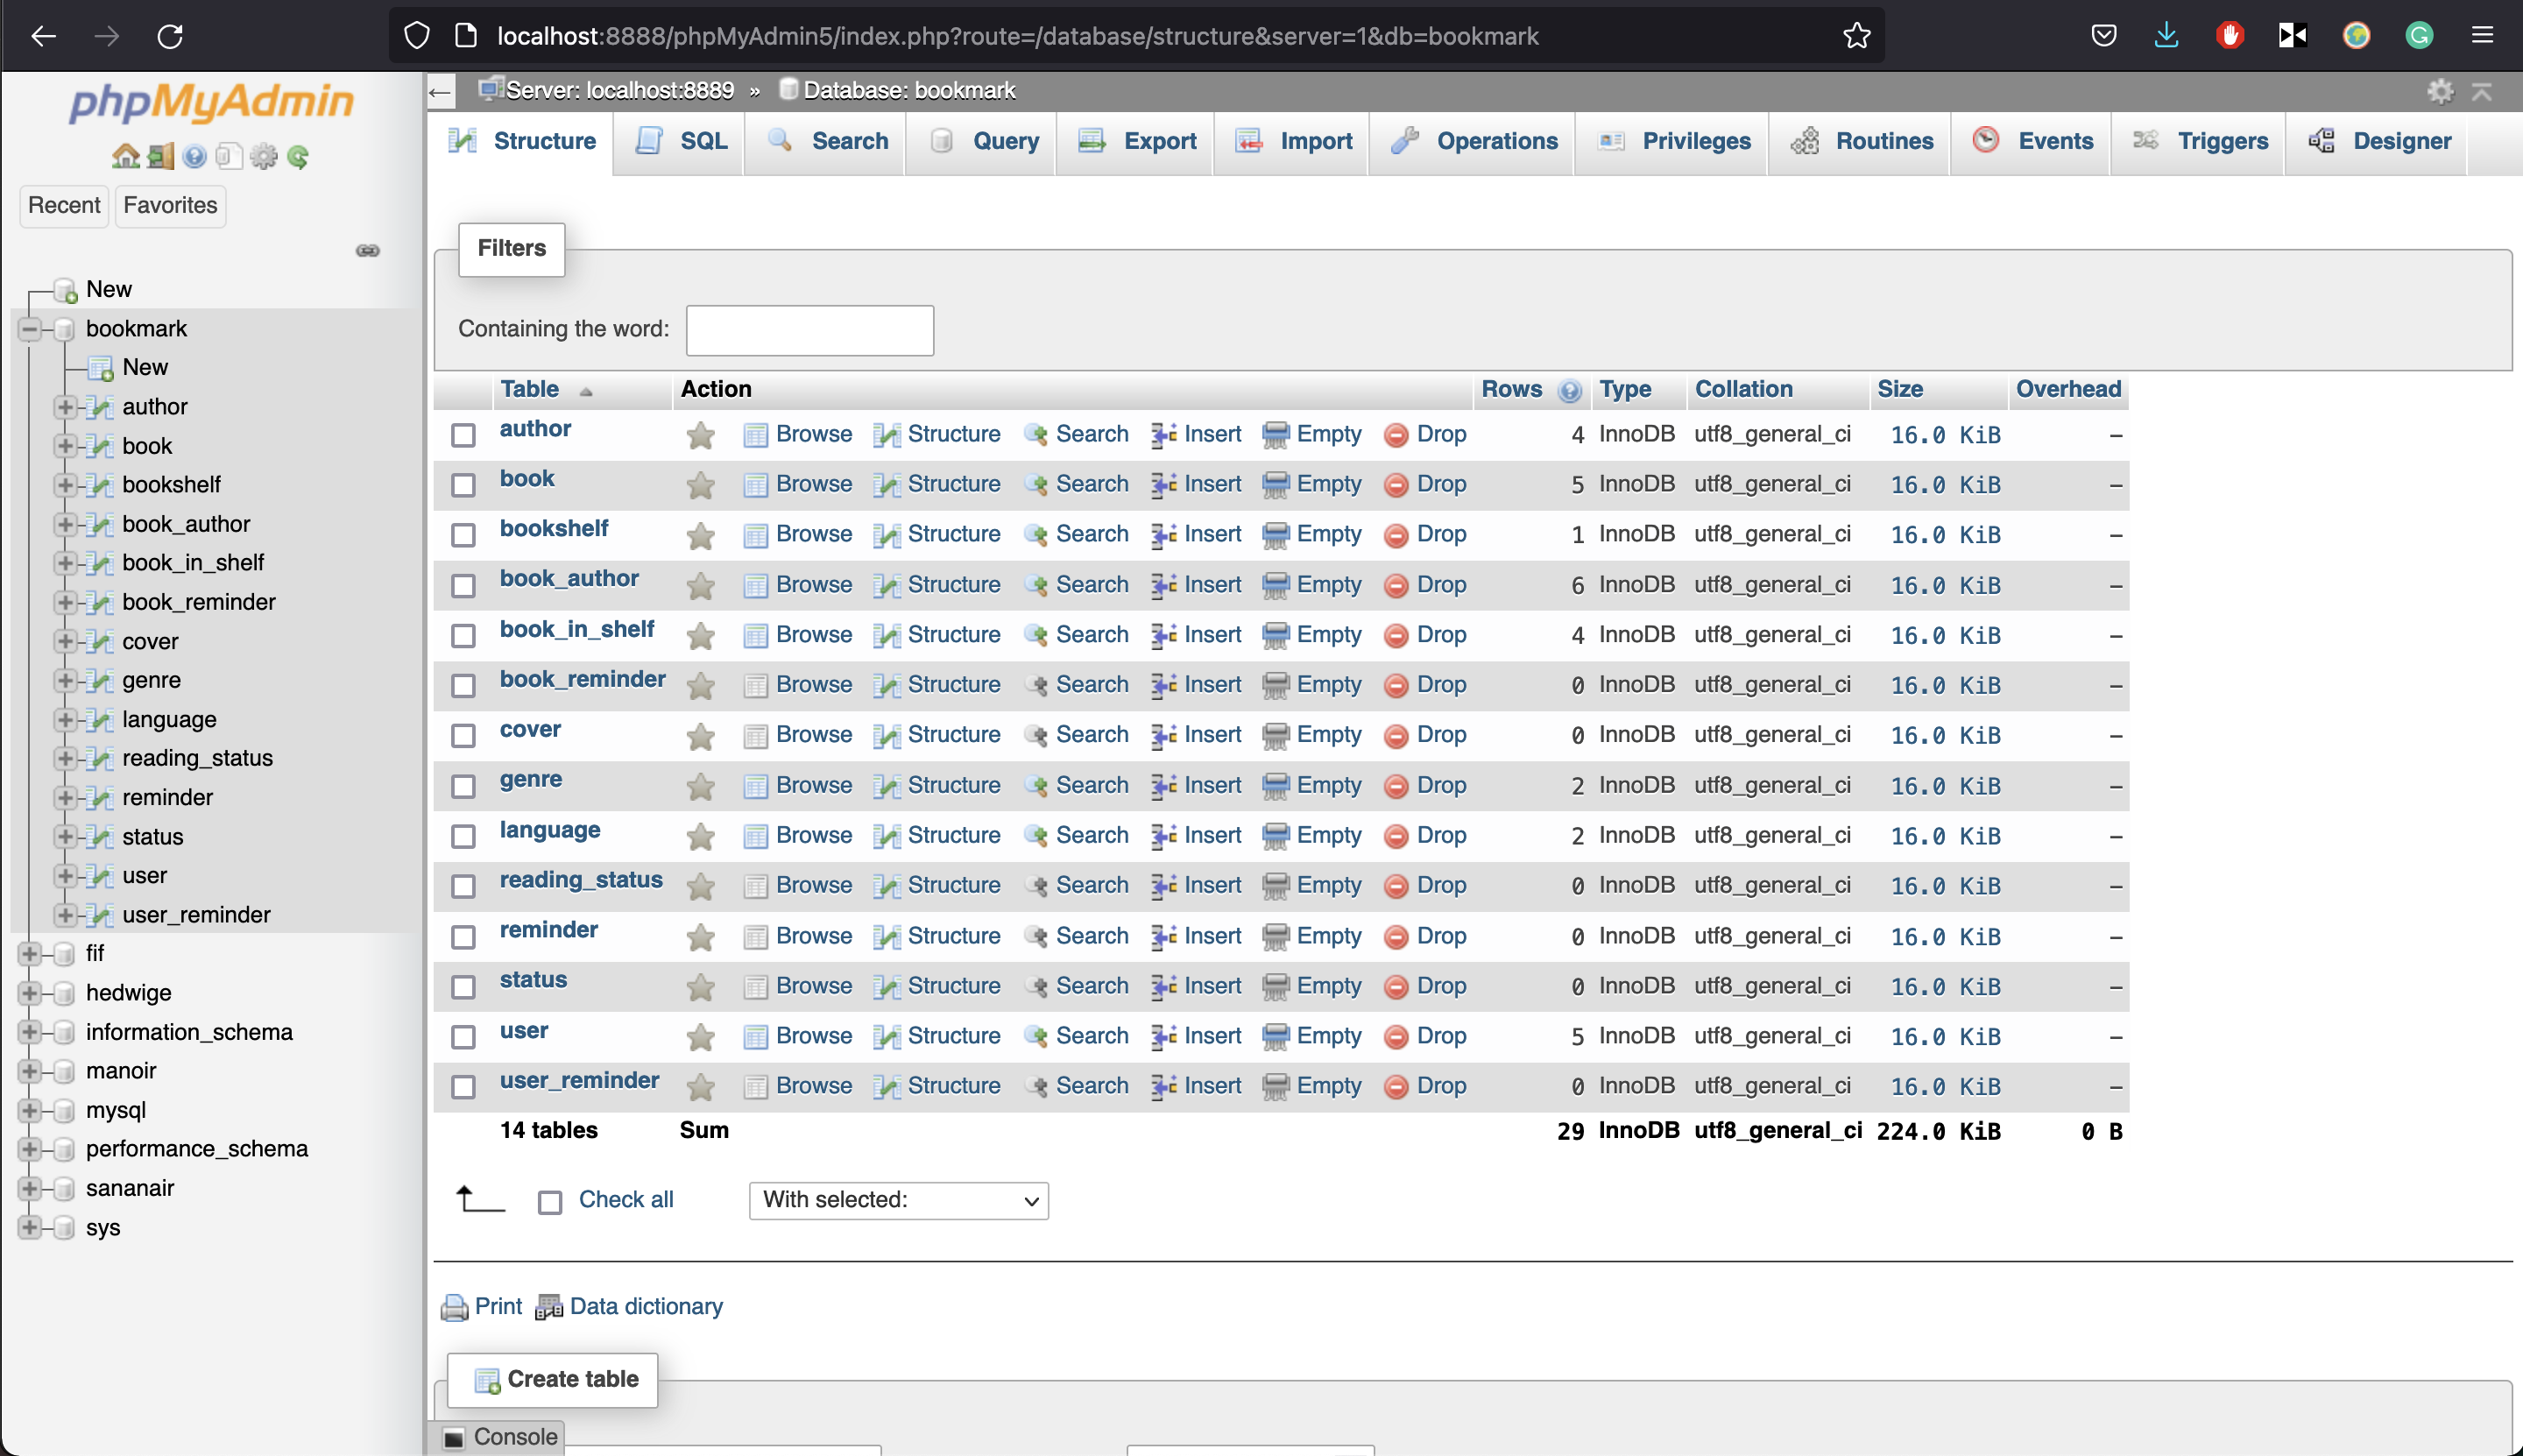
\includegraphics[width=\columnwidth]{Resources/Architecture/Database.png} 
    \caption{Local instance of the database}
    \label{fig:dblocal}
\end{figure}

\subsection{Module 2: API}

Since an application cannot directly send requests to a database (and since that wouldn't be secure), the API acts as an interface between the application and the database.
Our API is coded in object-oriented PHP, and can be required with the following URL format on the BookMark website:\\ \textit{/api/endpoint/param1/param2/...}\\
where endpoint is one of the three endpoints (user, book or bookshelf), and the parameters are sent to specify the requested action or provide additional data for the action. On the server, everything is redirected to the index page, and the URL is then parsed by a "router" file, that will split it with the '/'s and isolate each parameter in an array. The router file also gets the method of the request (GET, POST, PUT, etc.) and then calls the corresponding API endpoint.\\

The API in itself is an abstract class (Api) that contains all the methods for building a query, connecting to the database and sending the query. The endpoints book, user, and bookshelf extend the Api class (ApiBook, ApiUser, ApiBookshelf and ApiRecommend) and contain specific methods for parsing and handling the data they are given.\\
When initializing an instance of the class being called by the router, the router sends it the URL parameters in an array and the name of the method used in a string. This method is used to switch between different cases. These different cases call to the functions which process the data, and which in turn call the functions to send or fetch data from or to the database.\\
The API is based on a CRUD (Create, Read, Update, Delete) paradigm, so the inner functions are meant to perform only one of the four following actions. Depending on the method used, the method used will be different: for example a Get request will trigger a Read action, whereas a Patch request will trigger an Update action.

The outputs of the API are formatted in JSON and echoed simply in the page. The API can also return response codes if errors occurred during the processing of the request, the most common ones being Forbidden (403), Not Found(404) or Method Not Allowed (405). Otherwise the usual response code is the default code Ok (200).

\begin{center}
\begin{figure}[h]
    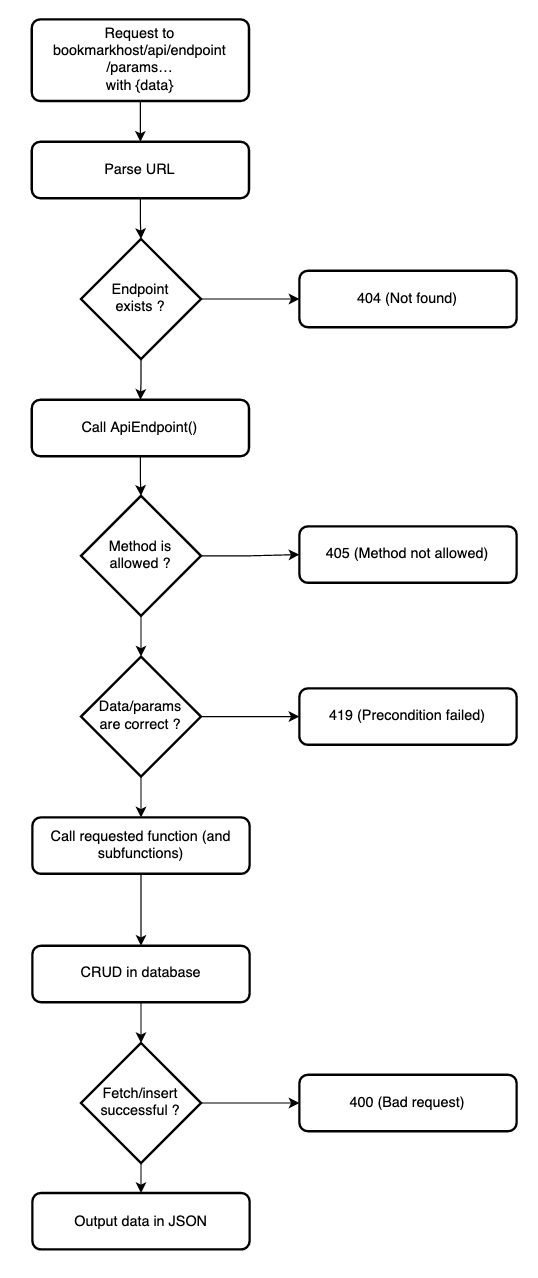
\includegraphics[height=1.8\columnwidth]{Resources/Architecture/API Module.png}\\
    \caption{API flowchart}
    \label{fig:apiFlowchart}
\end{figure}

\begin{lstlisting}[language=custom]
class ApiBook extends Api
{
    private $_response ;
    public function __construct ($url, $method)
    {
        switch (strtolower($method)) {
            case "get":
                $this->_response = $this->getBook($url) ;
                break ;
            default:
                $this->_response = $this->errorResponse("METHOD NOT ALLOWED") ;
                http_response_code(405) ;
        }
        echo json_encode($this->_response) ;
    }
}
\end{lstlisting}
\textit{Example of initialization for the book endpoint}
\end{center}

\subsection{Module 3: BookMark Application}

The frontend application is a Swift, iOS oriented app. Its purpose is to allow the user to manage his account, books and bookshelf from a graphical interface. We use Xcode as our development IDE, so at the creation of the project, the module is divided into three main folders: BookMark, with the main Swift code, BookMarkTests, comprising the data tests, and BookMarkUITests, with the graphical user interface tests. The main code itself is divided between views and models.\\

Models (Model.swift, Requests.swift and ModelEnpoints.swift) contain structures, functions and global variables that are used in all of the views. The ModelEndpoints Swift file contains the URL of the host as well as all the links to the different endpoints. The Requests model contains two major functions, \textit{requestWithBody()} and \textit{requestNoBody()}, that are used to build and send requests to the API. And finally, the Model file references all the structures and enums that are used in the app, like for example \textit{Book}, \textit{Bookshelf}, \textit{Shelf}, but also \textit{Sorting} and \textit{UsrData}. These structures are written to match the output of the API.\\
For the views, each Swift file is an independent view. The main "door" to the app is the BookMarkApp.swift file, which launches the app and toggles the HomeView. Then, from the HomeView, the connected user accesses the ContentView, which is in essence the My BookMark page. This page displays his books, sorted depending on his preference (genre, author, title, ascending or descending) and also contains a link to the RecommendedView. The RecommendedView displays books that are recommended for the user based on the recommendation algorithm. From this page, by clicking on the + button next to each book, the user can add the book to his bookshelf.\\

Each of the application views sends requests to the API by using one of the two request functions when loading, then parses the data with the Codable structures and displays it. Some of the elements of the view, like for example lists, can be updated or refreshed on their own as they can be altered by the user's actions.

\section{Use Cases}

\subsection{Installation}
When user searches on keywords like ‘Bookshelf’ in the Appstore, our application will be displayed. After downloading the application, the phone of the user will contain our application and it’s icon will be on the home screen.
\subsection{Activate the application}
If user touches the icon of our application, a Login page will be displayed. The user is then required to type in their account information. If the typed in account is correct and thereby exists in the database, a Main Page will be presented (If user does not have an account. They will need to press the key ‘Sign Up’. This will be presented later under “Sign Up”).
\subsection{Main Page}
The Main page is the first screen shown, after user have logged in to the application. After logging in, user is presented with multiple options in the Main page. The Main page has different categorized book sections like ‘New arrivals’, ‘Currently reading’, ‘Your category’, and ‘Suggestions’ lists. In these sections books are listed as their categories. ‘New arrivals’ will show new books added to the applications and highlight books that the user might be interested in. ‘Currently reading’ will show the books user is reading at the moment and where they are in the book. ‘Your category’ will display themes and genres of books and audiobooks that user might find interesting, and ‘Suggestion’ will show book suggestions based on what the user has read earlier. Also, you can search for books within the search box, proceed to your personal profile page, and log out.
\subsection{Tutorial of the application}
User will be presented with an optional tutorial of the application. If they choose the tutorial option, a simple description of how to use the application will show up on the screen. \\

\subsubsection*{a. Explanation of how to use the application}\hfill\\
\begin{enumerate}
    \item Choose a book that you would like to read. \\
    Tap the cover of the book or search for a specific book with the search function.
    \begin{itemize}
        \item In the ‘Search’-box, write the book title, author, or other keywords that you want to find books containing. \\
        When you’ve found the book you would like to read, type the title of the book and then tap the cover and move on to the ‘Add Book’ page. This page show’s the book title page and details like status(now reading or not), author, release date etc.
    \end{itemize}
    \item ‘Add To My List’ Button. \\
    Press this button to add the book to your personal reading list, for books you would like to read later.
\end{enumerate} \hfill\\
After reading the tutorial, user can make their own reading list(s), by searching or choosing the books in the Main page. \\

\subsubsection*{b. Main page}\hfill\\
\\
The application will make a collection of books, which will be suggested based on your preferences, search history, and other suggestions. New Arrivals, Now Reading, Your Categories and Suggested Books will be displayed with title and cover. You can see the ‘Add Book’ page showing detailed information about the book by touching the cover of the book, or you can search for books that you are looking for, and check your profile.
\begin{itemize}
    \item Person shaped Button \\
    If user touches this icon, they will get to their profile page - My bookmark.
    \item Book list Button \\
    Screen will show books divided into the categories: New arrivals, Now reading, Your selected category, Suggestions, based on what user is reading.
    \begin{itemize}
        \item New arrivals
        \item Currently reading
        \item Your category
        \item This is For You(Suggested)
    \end{itemize}
    \item Search \\
    By searching, user can find the books they are looking for (it links to a detailed search page)
    \item Logout \\
    After user is done using the application, they log out by pressing the ‘Logout’ button.
    \item[1)] User wants to add new book 
    \begin{itemize} 
        \item[1.1)] If the book is on the main page, user can select the book by touching the cover.
        \item[1.2)] If the book is not on the main page, user needs to search for the book.
    \end{itemize}
    \item[2)] When book cover is touched, ‘Add Book’ page will be displayed. The page has some detailed information about books like reading status, author, release date, total pages, etc.
    \item[3)] Tap ‘Add To My List’, and the selected book is added in user’s reading list. In the reading list, the ‘Add To My List’ button is then changed to ‘Delete From My List’.
\end{itemize}
\subsection{Sign Up}
When user has no account and touches the ‘Create account’ button in the ‘Login Page’, the ‘Sign Up’ page will be displayed. On this page, user can enter Username, Email, Phone number and Password. Afterwards, user touches the ‘Sign Up’ button, which completes the creation of user’s account. The application will then go to ‘Choose page’.
\begin{itemize}
    \item[1)] User enters name, email, phone number, password and checks two boxes (see description further down). Then touches the ‘Sign Up’ button.
    \begin{itemize}
        \begin{itemize}
            \item User name\\
            Type name.
            \item Email \\
            Type email.
            \item Phone Number \\
            Type phone number.
            \item Password \\
            Type password.
            \item The two checkboxes \\
            ▢ ‘Agree to terms and conditions’ \\
            ▢ ‘Agree to receive newsletter and other promotional content’
            \item ‘Terms and conditions’ \\
            ‘Accept terms and conditions’ checkbox. User can touch ‘Read terms and conditions’ or mark the checkbox in acceptance of the terms and conditions. This means that they have read and agree to the terms and conditions for making a profile in the BookMark application.
        \end{itemize}
        \item[1.1)] If user clicks ‘Terms and conditions’ it leads to page ‘Terms and conditions’ 
        \begin{itemize}
            \item[1.1.1)] ‘X’ button \\
		    To go previous page, you can tap X button
        \end{itemize}
        \item[1.2)] In this page, user can read content about the application’s terms and conditions.
        \item[1.3)] If user clicks ‘Agree’, screen goes back into ‘Sign Up’ page, and the list’s checkbox is checked
    \end{itemize}
    \item[2)] Choose at least 3 types of books that user like.
\end{itemize}


\subsection{Choose Page}

User has to choose at least 3 types of books he/she likes. There are some categories of books like Fantasy, Romance, Comedy, etc. User chooses preferred genres of books. This page is shown only one time when user signs up.
\begin{itemize}
    \item[a.] Back \\
    If user entered wrong account information, he can go back into previous page by touching this button
    \item[b.] Search \\
    If there is no keyword matching with user’s taste, you can search by clicking search box and typing what you want to search.
    \item[c.] Complete \\
    If user finished selecting over 3 types of books, user can go into Main page by touching ‘Complete’ button.
    \begin{itemize}
        \item[1.] If user clicks Complete button with under 3 types of books \\
        Pop up message will appear to screen with message that ‘you have to select at least 3 types of books’
    \end{itemize}
\end{itemize}

\subsection{Log In}
\begin{figure}[h]
    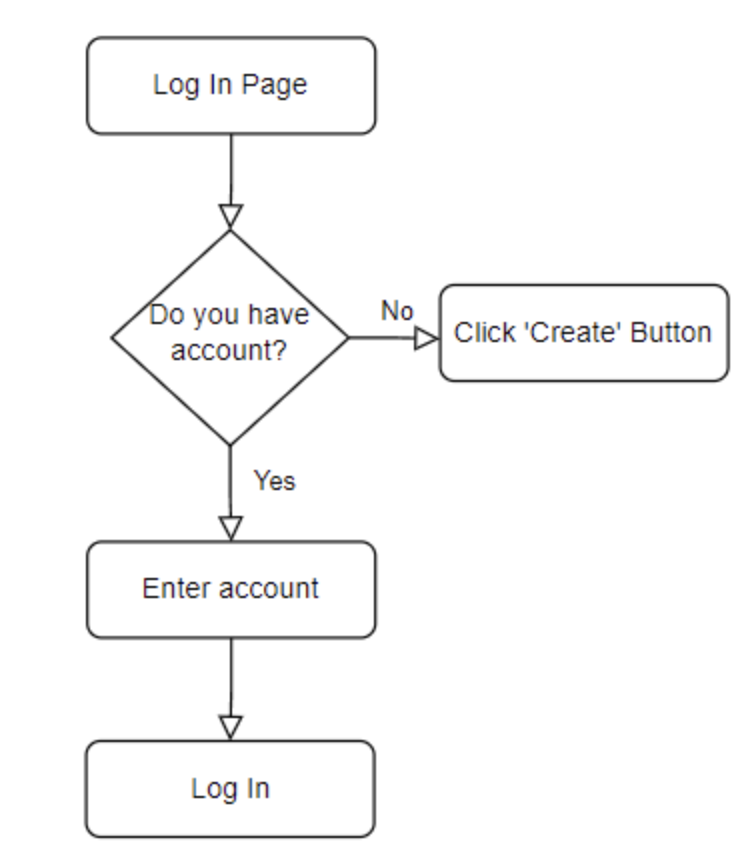
\includegraphics[width=\columnwidth]{Resources/login.png} 
    \caption{Login Use Case}
    \label{fig:login}
\end{figure}

\begin{itemize}
    \item[1)] Enter ID and password \\
    User must type in their existing ID and correct password. By default, user’s password is hidden and characters are shown as asterisks (*),  but by touching the ‘Show’ button the characters are displayed. If user forgets their ID and password, they can get them send to their email by clicking the button ‘Forgot your password?’
    \begin{itemize}
        \item[a.] If the user’s ID and password exist: login successful and move on to the main page.
        \item[b.] If the user’s ID and password do not exist: Pop up screen indication that login failed
    \end{itemize}
    \item[2)] Log In button
    \item[3)] Find ID and password \\
    If user does not remember their own ID or password, they can get send a message to their registered email. If the email address that user enters matches one that exists in the database, user will receive an email which shows ID and a link that will lead to a page where user can reset their password. If the entered email address does not match one in the database, the application will display a pop up with a message saying; ‘Sorry, the email that you have entered does not exist’.
    \item[4)] Sign In \\
    If the user has no existing account in the application, he/she needs to click Sign In, and make an account.
\end{itemize}

\subsection{Profile}
User can go into their profile page by touching ‘Settings’ or clicking the person-shaped icon in the Main page. In this page, user can see their Profile Picture, Username, Address, Now reading and Purchased books.
\begin{itemize}
    \item[1)] User’s profile picture \\
    User can select their own profile photo by clicking the default circle. If user clicks the circle, a pop up will appear with a message asking them to change the photo.
    \begin{itemize} 
        \item[1.1)] Changing photo \\
        If user selects ‘Change photo’, he/she has to choose a photo in his/her gallery. When user has done this, the profile picture is changed and action is complete.
    \end{itemize}
    \item[2)] Username and address is personal information. The Username is needed to make user’s profile personal. The address is needed if user would like books shipped to their address. This information can be edited in the ‘Settings’ page’ or the ‘Account’ page. This information cannot be changed in the ‘Profile’ page.
    \item[3)] My books \\
    The page shows all the books that the user has purchased. If there are no purchased books, it will display nothing. User can scroll if there is not enough screen to display all the books.
    \item[4)] Now Reading \\
    If user clicks the ‘Now Reading’ icon, it shows books that the user is currently reading. By clicking books, it shows the page where the user left off.
    \begin{itemize} 
        \item[3.1 & 4.1] Touching a book’s cover \\
        This page’s showing method is the same in the ‘My books’ and ‘Now reading’ pages.
        \begin{itemize} 
            \item[1.] If the book is the one that user is currently reading, it goes into ‘My Books’ page, user can keep reading or delete in the list.
            \item[2.] If user touches books cover and that is not read yet, It goes into ‘My Books’ page and user can start reading by touching start reading button
        \end{itemize}
    \end{itemize}
    \item[5)] ‘+’ button (adding books) \\
    From the profile page, by touching the ‘+’ icon, user will be moved to a searching page. Here user can add books to their reading list.
    \item[6)] ‘Back’ \\
    By touching the ‘Back’ button, user goes back to the previous page until they are at the Main page.
    \end{itemize}
    
\subsection{My Books (detailed)}
By touching the ‘My Books’ button the screen will show the books that user have bought. Here user can check the book's information, keep reading or remove it from the list.
\begin{itemize}
    \item[1)] Keep reading \\
    If user clicks this button, the application goes to the page of the book that you read last.
    \item[2)] Remove \\
    To remove a book from the reading list, clicking the button ‘Delete’. The application will the show an alert message and ask if user is sure that they would like to delete. If user clicks ‘Yes’ the book will be removed from their list. If user clicks ‘No’ they will go back to the ‘My Books’ page.
    \item[3)] Book information \\
    By clicking ‘Book information’ when selecting a book from the ‘My Book’ page, user will get information about the book. This can be general information like year of release, author, how many users have purchased this book, rating and more. 
\end{itemize}    

\subsection{Settings}
\begin{itemize} 
    \item[1)] Profile \\
    By clicking the ‘Profile’ button, the application will go to the Profile page
    \item[2)] My Account \\
    If user clicks ‘My Account’,  the application will go to the User Account page. It shows some detailed information about the user. The information is what user entered when they signed up.
    \begin{itemize}
        \item[-] Name
        \item[-] Phone
        \item[-] Email
        \item[a.] Reading Frequency
        \item[b.] Delete Account \\
        By clicking this, a pop up will be displayed, which asks if user wants to delete the account. If user clicks ‘Yes’, then the account is deleted, if user clicks ‘No’, it goes back to the previous page.
        \item[c.] Change information \\
        If user needs to change their own information, it can be changed by clicking the ‘Change Information’ button. A similar screen to the ‘Sign Up’ page will be displayed, where the user can edit their personal information.
        \item[d.] Settings \\
        If user clicks the ‘Settings’ button, the application goes back into the Settings menu.
        \item[e.] Logout \\
        If user clicks the ‘Logout’ button, a pop up will ask whether they really want to log out or not. If the user clicks ‘Yes’,  the application will go to the ‘Login’ page, and if they press ‘No’  the pop up will disappear. 
    \end{itemize}
    \item[3)] Mileage \\
    Whenever user buys a book, they earn mileage proportional to its price. You can check your mileage by clicking the Mileage block.
    \item[4)] Bookshelf \\
    When user wants to change settings of the bookshelf itself, it can activate by clicking this box. For example, changing user’s genre preferences is one of them
    \item[5)] Dark / Light Mode \\
    The user can change the mode of his screen (dark or light mode) and set all the reading notifications. A switch will be available for the user if he wants to activate or deactivate reading notifications is activated by default
    \item[6)] Language \\
    The user can select their preferred language for the application. The default language is English. After changing the language, all text in the application will change, as well as book suggestions will be in the language according to the selected language.
    \item[7)] Notifications \\
    In this part, user can set up their own notification preferences. They can choose their preferred notification settings, reading reminders and marketing content.
    \item[8)] Delete Account \\
    To delete the account, user has to click the ‘Delete Account’ button. After clicking the button, a pop up message will appear inquiring whether they really want to delete their account. If they click ‘yes’, all data of the account will be deleted and if not, the pop up will disappear. 
\end{itemize}








\begin{thebibliography}{00}
\bibitem{RFID} 
\url{https://gzandea.en.ecplaza.net/products/rfid-smart-bookshelveshf-intelligence-bookshelffile-management_3914989}

\bibitem{Smartbookshelf}
\url{https://www.red-dot.org/ko/project/smart-ai-modular-bookshelf-26628}

\bibitem{Goodreads}
\url{https://www.goodreads.com/}

\bibitem{Bookbrowse}
\url{https://www.bookbrowse.com/}

\bibitem{Storygraph}
\url{https://www.thestorygraph.com/}

\bibitem{LDM}
\url{https://drive.google.com/file/d/1qXDdPbP0vvrqVYIyJdMQ6C-DeG7IgjeZ/view?usp=sharing}

\end{thebibliography}





\end{document}